\chapter{Data Manipulation}

\section{Manipulating Geometrical Data}
\index{Manipulating geometrical data}

There is a small number of function to manipulate geometric data in \ogs. The common approach to the manipulation of \ogs input data is that it should be changed in a GIS or other specialised software of the user's choice which usually offers much more functionality for these things than \ogs ever could.

However, it is possible to set or change names for any geometrical object by right-clicking on the object and selecting \cmd{Set name...}\index{Setting names}\index{Changing names}. Upon saving the data again, the new or modified names will be saved in the corresponding file.

Functions for the actual manipulation of geometric data that \emph{are} implemented are all associated with polylines and can be applied by right-clicking the ``Polylines'' item of any geometry and selecting \cmd{Connect Polylines...}.

\subsubsection{Connecting Polylines}
\index{Connecting polylines}
This function connects all the selected polylines to a single new polyline provided that the start- and end points of all segments are within the given maximum distance. The default maximum distance is $0.0$, meaning that start- and end points have to be identical.

Note that if more than two start/end points are located within the given maximum distance, still only two of those points are connected. These points are chosen randomly.

\subsubsection{Creating Polygons by Closing Polylines}
\index{Creating polygons from polylines}
This function closes a (connected) polyline. Simply check `Close connected Polyline'. If a name has been entered, this name will be assigned to the closed polyline.

\subsubsection{Creating Surfaces by Triangulating Polygons}
\index{Creating surfaces from polygons}
This function additionally creates a new surface by triangulating the polygon. This simply requires checking `Create Surface from Polyline'. The newly created polyline has to be closed for that function to work. If a name has been entered, this name will be assigned to the surface.

\section{Creating Meshes from Geometry}
\label{meshcreation}\index{Creating meshes}

By selecting \cmd{Tools\ra Mesh Generation...} a dialogue that allows the user to create meshes using information currently present in the programme. For this to work, the open-source mesh generating software GMSH\footnote{http://geuz.org/gmsh/} needs to be installed and be available from the location of the Data Explorer (i.e. located in the same directory or findable, e.g. via PATH-variable under MS Windows).

The user can select any geometry and observation sites that should be considered for generating the mesh. Note that all points of every data set considered for mesh generation will be included as nodes in the final mesh. Therefore it makes sense to check if succeeding points of polylines are unnecessarily close together or too far apart. It is furthermore necessary that at least on polyline in any of the selected geometries is closed (i.e. is a polygon). Any polygons found in the geometry will be meshed, polygons within polygons will simply be integrated within the encompassing larger shape.

Upon pressing \cmd{OK} a geometry-file (*.geo) for GMSH is written, GMSH is called to create the mesh and the newly created mesh is at once imported in the \ogs-Data Explorer.

There is an \cmd{Advanced}-Tab in this dialogue that allows to set a number of parameters for the mesh. Most importantly, it can be chosen, if the new mesh should be adaptive or homogeneous. An adaptive mesh{Adaptive Meshes} is refined towards points or lines specified in the geometry while a homogeneous mesh has elements of roughly the same size everywhere in the domain (see figure \ref{fig:meshing}).

\begin{figure}[tb]
\begin{center}
\subfloat[Geometry]{\includegraphics[width=0.3\linewidth]{meshing-geo}\label{meshing-geo}}\enspace
\subfloat[Homogeneous mesh]{\includegraphics[width=0.3\linewidth]{meshing-hmg}\label{meshing-hmg}}\enspace
\subfloat[Adaptive mesh]{\includegraphics[width=0.3\linewidth]{meshing-adp}\label{meshing-adp}}
\end{center}
\caption{Meshing using geometric data and observation sites.} \label{fig:meshing}
\end{figure}

The specific parameters for adaptive meshes are:
\index{Adaptive meshes}
\begin{itemize}
\item \textbf{Max. number of points in Quadtree leaf:} Generally speaking, the smaller this number the finer will the resulting mesh be. \\
    To be more exact, you have to have a basic idea what a quad tree \footnote{http://en.wikipedia.org/wiki/Quadtree} is: A tree structure is constructed by a sequential subdivision of the domain based on the distribution of relevant points in space. The criterium if a segment compromising a leaf is further refined is dependent on the number of points located within that segment. Therefore, larger numbers of that parameters will usually result in coarser meshes while smaller numbers will result in finer meshes. \emph{Note that this is technically not a correct explanation as results are heavily dependent on how many points are located in certain sub-divisions of the domain, the existence of point clusters, etc.} See figure \ref{fig:quadtree} for an example.
\item \textbf{Mesh density scaling for points:} This is a scaling factor for the above parameter allowing for a refinement towards points located within the outer boundary. Again, smaller values will result in finer meshes.
\item \textbf{Mesh density scaling for stations:} This is exactly the same kind of scaling factor as for the option above, only for refinement towards observation sites, allowing a different mesh density for different regions of the mesh.
\end{itemize}

\begin{figure}[tb]
\begin{center}
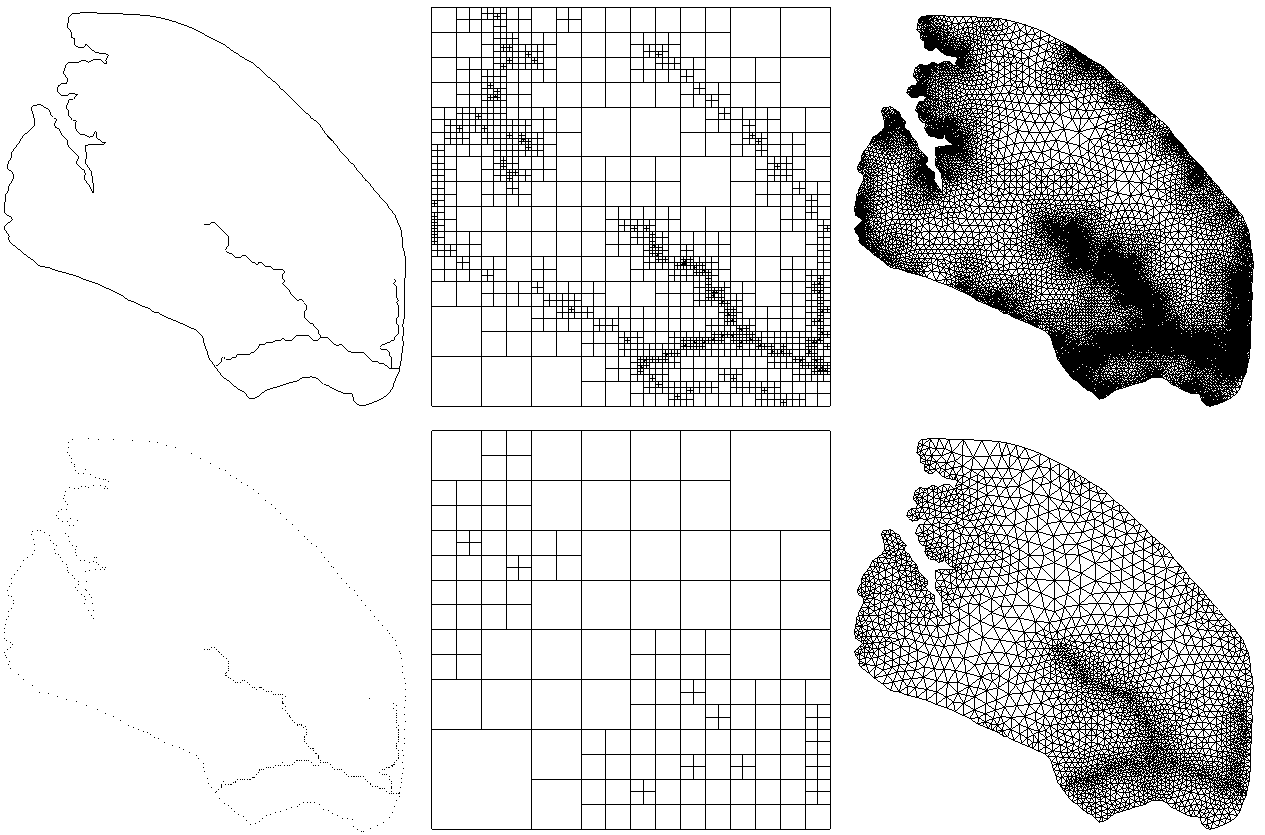
\includegraphics[width=0.95\linewidth]{quadtree}\label{quadtree}
\end{center}
\caption{Adaptive meshing of geometry. The left colomn depicts polyline and points that need to be meshed. In the middle the resulting quad trees can be seen, the upper on generated with a maximum of two points per leaf, the lower one with 10 points per leaf. The resulting meshes are shown on the right side. Notice that regions where no information is available have roughly the same element size while elements where point information is given differ vastly in element size.} \label{fig:quadtree}
\end{figure}

Likewise, you can select an \textbf{element size}\index{Element size} for homogeneous meshes.\index{Homogeneous meshes} Here, too, a smaller number will result in a finer mesh, as the value specifies the maximum edge length of mesh elements.

\bigskip

Default parameters for all options are already predefined and have worked well with most examples that have been tested. Feel free to play around with these numbers but realise that the resulting mesh might not be what you have in mind.

\section{Creating Meshes from Raster Files}
\label{meshraster}\index{Creating meshes}

\begin{figure}[tb]
\begin{center}
\subfloat[Raster]{\includegraphics[width=0.3\linewidth]{rastermesh1}\label{rastermesh1}}\enspace
\subfloat[Elevation]{\includegraphics[width=0.3\linewidth]{rastermesh2}\label{rastermesh2}}\enspace
\subfloat[Materials]{\includegraphics[width=0.3\linewidth]{rastermesh3}\label{rastermesh3}}
\end{center}
\caption{Creating meshes from raster files: Pixels can be either represented as a set of two triangles (Fig. \ref{rastermesh2}) or a square (Fig. \ref{rastermesh3}), intensities may represent elevation (Fig. \ref{rastermesh2}) or materials (Fig. \ref{rastermesh3}).}
\label{fig:rastermesh}
\end{figure}

A completely different way to create a mesh is based on image or raster files, such as *.asc-files from ArcGIS. If the file is loading into the Data Explorer it will appear in the visualisation pipeline only. Right clicking the object allows to select the menu item \cmd{Convert Image to Mesh...}. A dialogue allows the parameterise how exactly this conversion should be performed. Specifically, it is possible to select a mesh element type for representation of pixels and a way in which grey-values should be interpreted\footnote{Meshes can also be generated from colour images. However, the colours will be converted to grey-values via $g = 0.3*\text{red}+0.6*\text{green}+0.1*\text{blue}$.}.

For the first parameter, pixels can be converted into a square (i.e. a quadrilateral element) or two rectilinear triangles (i.e. two triangle elements). In the future it is also planned to offer cubes (i.e. a hexahedron) for multi-layered images.

For the second parameter the user can decide pixel values should be interpreted as elevation (which is useful if the raster represents a digital elevation model) or if the grey-values should be assigned as scalar values to the mesh elements. As an alternative, these values can also be ignored (see Fig. \ref{fig:rastermesh} for examples).

If the raster file contains ``NoData''-values (this is common in raster files created with a Geographic Information Systems such as ArcGIS), these values are ignored and will after the conversion not appear as mesh-elements (i.e. despite the raster file always being rectilinear the resulting mesh may have an arbitrary boundary defined be pixels actually containing information).

\section{Extruding Meshes to 3D}
\index{Extruding meshes}

Any 2D mesh loaded into \ogs can be extruded into a 3D mesh by copying the 2D mesh layer a specified number of times and then connected any two neighbouring layers by creating 3D elements from all corresponding 2D elements (i.e. two triangles are connected and form one prism-elements, two quadrilateral elements form one hexahedron). This functionality can be accessed by right-clicking on a mesh in the data view and selecting \cmd{Edit Mesh...}. In the \cmd{3D Extrusion}-tab of the resulting dialogue the number of mesh layers and the distance between neighbouring layers can be specified.

\section{Mapping of Meshes based on DEMs}
\index{Mapping meshes}

For assigning elevation profiles to each layer, select the \cmd{Layer Mapping}-tab. Here, for each layer of the mesh a raster file in *.asc format can be selected and will be assigned to the respective mesh layer. Note that not for every layer a DEM file need to be specified. If no file path is given the mapping of the layer is simply skipped.

\begin{figure}[tb]
\begin{center}
\subfloat[Surface Mesh]{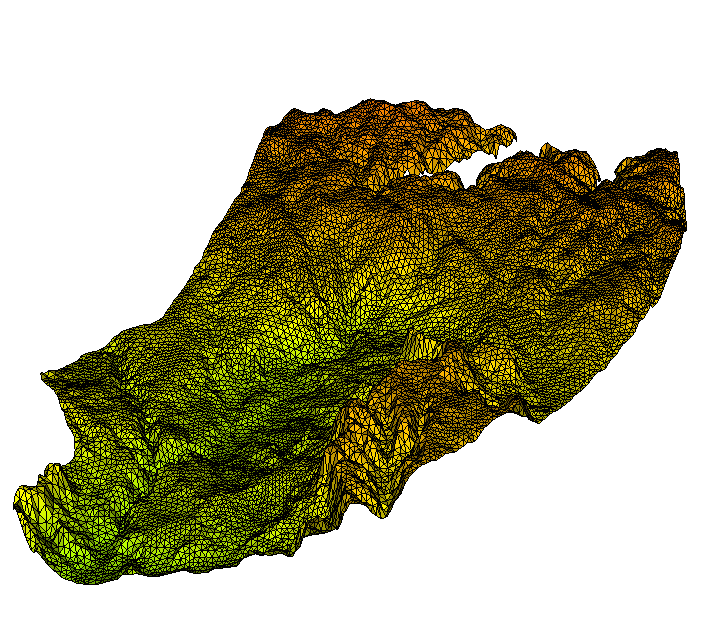
\includegraphics[width=0.3\linewidth]{AmmerSurface}\label{fig:AmmerSurface}}\enspace
\subfloat[Subsurface Layers]{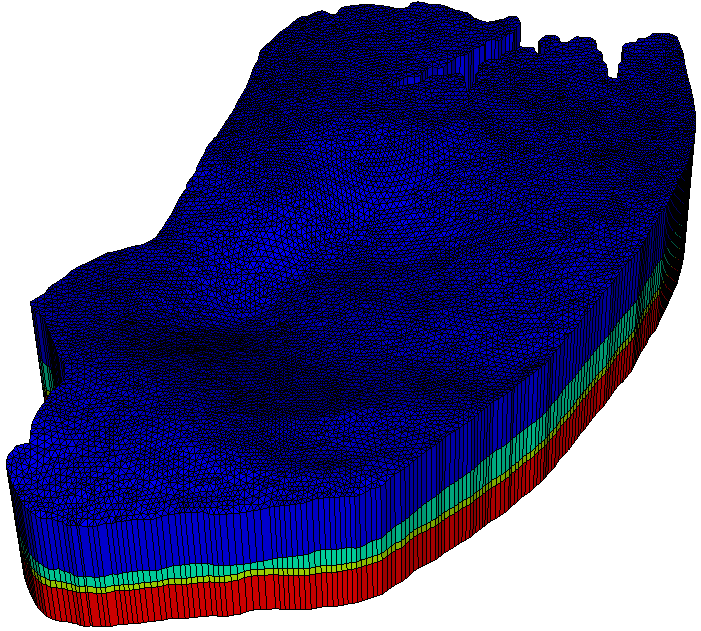
\includegraphics[width=0.3\linewidth]{AmmerSubsurface}\label{fig:AmmerSubsurface}}\enspace
\subfloat[Final Mesh]{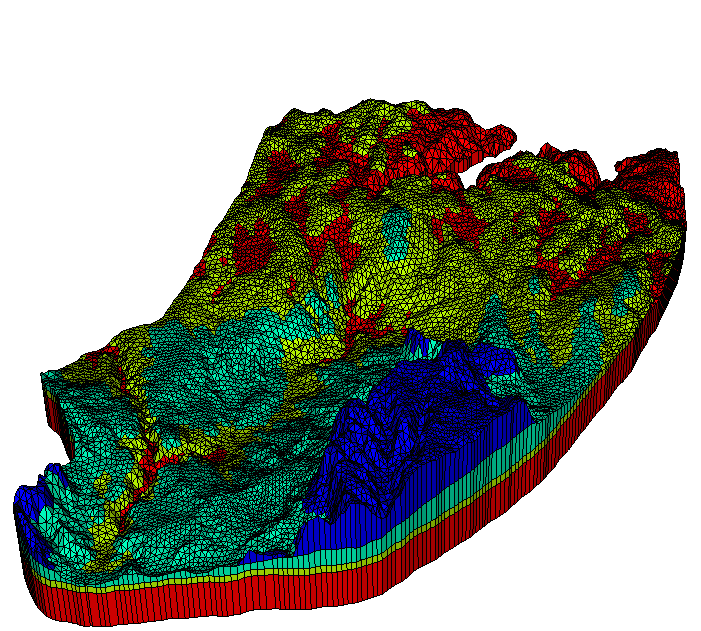
\includegraphics[width=0.3\linewidth]{AmmerFinal}\label{fig:AmmerFinal}}
\end{center}
\caption{Mapping meshes based on raster files: A surface mesh is extruded and four layers are added. These subsurface layers are mapped according to elevation models. In a final step the subsurface model is intersected with the terrain model.}
\label{fig:RasterMapping}
\end{figure}

For multi-layered meshes the mapping will first be performed on all subsurface layers and the resulting mesh will then be intersected with the DEM-layer (i.e. the digital terrain model), thus effectively cutting away all elements located above surface. \emph{Note that currently the check if two layers are intersecting each other does \emph{not} work correctly for any other layers except the DEM!}

For meshes containing only 2D elements there is also an option ``Remove mesh nodes at NoData values''. Per default this option is switched off as it is dependent on the meshing if the result will be topologically correct.


\section{Analyse Mesh Quality}
\index{Mesh quality}

You can visualise the quality of a given mesh by right-clicking on the mesh in the respective data view and selecting \cmd{Check Mesh Quality...}. This allows to choose between currently four implemented measurements for mesh element quality. The result of choosing any of these modes is a colour-codes overlay of the mesh where every element is assigned a quality in $[0,1]$. You can select this overlay in the visualisation pipeline and specify thresholds to select a certain range of quality and see which element fall into that range. \emph{(Note: You might need to manually set the correct scalar array for visualising mesh quality. The appropriate data can be chosen by selecting in ``C-Selection'' in the \cmd{Active Scalar} pull-down menu.}

\begin{figure}[tb]
\begin{center}
\subfloat[Edge Aspect Ratio]{\includegraphics[width=0.3\linewidth]{MshQualEdgeRatio}\label{fig:mshqual1}}\enspace
\subfloat[Element Area]{\includegraphics[width=0.3\linewidth]{MshQualArea}\label{fig:mshqual2}}\enspace
\subfloat[EquiAngle Skewness]{\includegraphics[width=0.3\linewidth]{MshQualEquiAngle}\label{fig:mshqual3}}
\end{center}
\caption{Examples for colour coded mesh quality measurements.} \label{fig:mshqual}
\end{figure}

The currently implemented measures are the following:
\begin{itemize}
\item \textbf{Aspect Ratio of Edge Length:} Analyses the ratio of shortest to longest edge of every element. Equilateral elements are often considered superior and better suited for FEM simulation, therefore these elements are rated ``1'' with their quality degrading with increasing differences in edge length. Each element is assigned the value of the highest ratio between any two of its edges. This is a good measure for triangle elements but might be not as good as others. See figure \ref{fig:mshqual1}.
\item \textbf{Area of 2D Elements:} Compares the area of all 2D elements (this includes the faces of 3D elements!) by assigned ``1'' to the element with the largest area and ``0'' to the element with the smallest area. See figure \ref{fig:mshqual2}.
\item \textbf{Volume of 3D Elements:} As with the area-criterion, this measure compares the volume of 3D mesh elements. 2D elements are ignored when this option is selected.
\item \textbf{Angles between Adjacent Edges:} Calculates the maximum deviation of an angle between any two adjacent edges of the element from the ``optimum'' angle, i.e. the angle of an equiangular element. This optimum angle is $90\degree$ for triangles or tetrahedra and $90\degree$ for quadrilateral or hexahedral elements. This measurement is called \emph{EquiAngle Skewness} and given by
    \begin{equation}
    s = \max\left[\frac{\theta_{max}-\theta_{opt}}{180-\theta_{opt}},\frac{\theta_{opt}-\theta_{min}}{\theta_{opt}}\right]
    \end{equation}
    where $\theta_{max}$ is the maximum angle between any two edges found in the element, $\theta_{min}$ is the minimum angle and $\theta_{opt}$ is the optimum angle.
    See figure \ref{fig:mshqual3}.
\end{itemize}

The quality measure best suited for a given mesh might depend on the process you want to simulate using this mesh. For instance, processes such as groundwater recharge consist mainly of layered flows, meaning that large differences between horizontal and vertical element surfaces might have no effect on a correct result. The simulation of mass transport processes explicitly requires a fine mesh resolution in vertical direction to ensure a stable solution.

\section{Creating Processes}
\index{Creating processes}

It is possible to add processes to the workflow in the Modelling-tab by pressing the \cmd{Add process...}-button. A dialogue will open that allows to select a process type and an associated primary variable. As of version 5.2.07 this has no effect except for boundary conditions being grouped under these processes and being removed upon removing the process (via right-click \cmd{Remove process}).

\section{Creating FEM Conditions}
\index{Creating FEM conditions}
\index{Creating boundary conditions}

It is possible to create FEM conditions based on geometric objects. By right-clicking on the respective point, polyline or surface and selecting \cmd{Set as FEM condition...} a setup dialogue will open (Fig. \ref{fig:CondSetupDlg}). Here, it can be specified for which process and primary variable the condition should be used and if it should be a boundary condition, a source term or an initial condition. Based on the geometrical object type and the selection of the condition type a number of distribution types will be available. For example, points as boundary conditions can only have \emph{Constant (Dirichlet)} distribution; lines as source terms can have \emph{Constant (Neumann)} or \emph{Linear (Neumann)} distribution, etc.

\begin{figure}[tb]
\begin{center}
\subfloat[FEM Condition Setup]{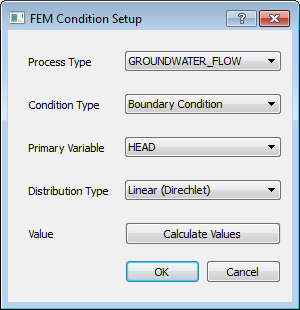
\includegraphics[height=4.0cm]{dlg_cond_setup}\label{fig:CondSetupDlg}}\enspace
\subfloat[Linear]{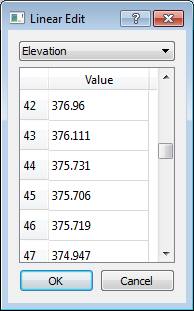
\includegraphics[height=4.0cm]{dlg_lin_dist}\label{fig:LinearDlg}}\enspace
\subfloat[Direct]{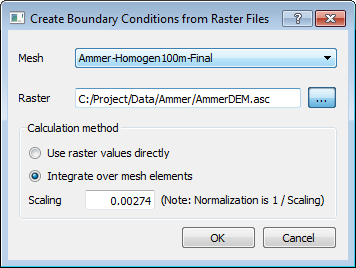
\includegraphics[height=4.0cm]{dlg_direct_dist}\label{fig:DirectDlg}}
\end{center}
\caption{Dialogues for creating of FEM Conditions.} \label{fig:CondSetup}
\end{figure}

While the assignment of values is easy for \emph{constant} distributions, it an get quite complex for \emph{linear} or \emph{direct} distributions. The FEM Condition Setup Dialogue will therefore contain a button ``Calculate Values'' instead of a textfield. Upon pressing this button a (different) dialogue will open to configure the values. For \emph{linear} distributions a table is displayed where for each point of the line a value can be inserted (Fig. \ref{fig:LinearDlg}). Conditions are only actually set up between points with given values. As an alternative it is possible to automatically insert the elevation (z-Coordinate) for each point of the line. For \emph{direct} distributions the dialogue will require to specify a raster file from which values are read for direct assignment to mesh nodes (Fig. \ref{fig:DirectDlg}). The user can select between a 1:1 assignment or a surface integration based on the area of the mesh elements the respective node is part of. In this case it is also possible to specify a scaling value to compensate for data files with different units of measurement.

For polylines or surfaces it is also possible to assign the conditions not directly on the geometric objects but instead on all points compromising the object. For example, a polyline consisting of 50 points can be either assigned one boundary conditions with a linear distribution or 50 boundary conditions on the respective points, each of which has a constant value.

Once created, FEM conditions can be saved by right-clicking associated process in the ``Modelling'' tab and selecting \cmd{Save FEM conditions...}. The user can specify the file format (XML or ASCII) and the type of conditions that should be written (boundary conditions, initial conditions, source terms or all of them).

\section{Changing FEM Conditions}
\index{Changing FEM conditions}

Conditions loaded into the \ogs Data Explorer can be edited simply by right-clicking the respective geometric object in the ``Modelling'' tab and selecting \cmd{Edit condition}. This will once again open the FEM Condition Setup Dialogue that is also used for creating conditions. For existing conditions the appropriate values will already have been selected and can now be changed. Changes in the corresponding files will only be written once the user actively saves these files again via \cmd{Save FEM Conditions...}

\section{Time series data and stratigraphic data}
\index{Time series data}\index{Stratigraphic data}

For observation sites it is possible to display additional information such as logger data at the site or the stratigraphy at a borehole. Both features are currently only implemented as a proof of concept and need to be expanded in the future.

To view the additional information of an observation site load a stn-file into the programm and right-click on any observation site in the data view. You will see either the menu entry ``View Stratigraphy...'' for a borehole or ``View Diagram...'' for a station. If you selected to view a diagram, a dialogue will open which allows you to select a start and end date or to load a file that contains the data (if no associated data base entry for the station has been found). A new window will open, displaying the requested information.

